% magick -quality 90 -density 1200 $input $output

\documentclass{standalone}
\usepackage{tikz}

\usetikzlibrary{calc,math}


\begin{document}

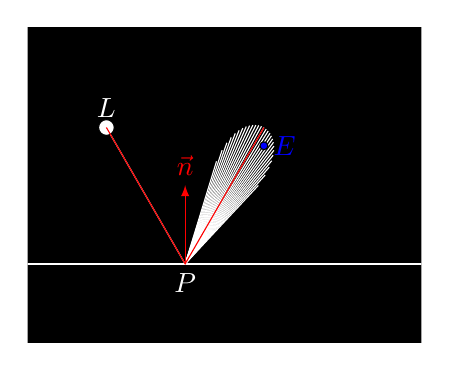
\begin{tikzpicture}
  \path[clip] (-2,-1) rectangle (3,3);
  \draw[fill=black,black] (-2,-1) rectangle (3,4);
  \draw[thick,white] (-3,0) -- (4,0);

  \coordinate (hit) at (0,0);
  \coordinate (light) at ($ (hit) + (120:2) $);
  \coordinate (eye) at (1,1.5);

  \draw[white] (light) -- (hit);
  \foreach \x in {47,...,73} {
    \tikzmath{
      real \r;
      \r = 2 * cos(abs(60-\x) * 3.14159265 * 2) ^ 0.2;
    }
    \draw[white] (hit) -- (\x:\r);
  }

  \draw[fill=blue] (eye) circle [radius=0.05cm] node[right,blue] {$E$};
  \draw[fill=white] (light) circle [radius=0.1cm] node [white,above] {$L$};
  \node[anchor=north,white] at (hit) {$P$};

  \draw[red,-latex] (hit) -- ++(0,1) node[above] {$\vec n$};

  \draw[red] (light) -- (hit) -- (60:2);
\end{tikzpicture}

\end{document}